\begin{frame}[fragile]{CNN - Convolutional Layer}
\begin{block}{Operation:}
    \begin{itemize}
        \item Element‑wise multiply filter with image patch and sum → feature map.
    \end{itemize}
\end{block}

\begin{block}{Hyperparameters:}
    \begin{itemize}
        \item kernel size
        \item number of filters
        \item stride
        \item padding
    \end{itemize}
\end{block}

\begin{lstlisting}[language=Python, caption={Code snippet (PyTorch)}, basicstyle=\ttfamily\footnotesize]
import torch.nn as nn

conv = nn.Conv2d(in_channels=3, out_channels=16, kernel_size=3, stride=1, padding=1)

output = conv(input_tensor)  # input_tensor: [batch_size, 3, H, W]
\end{lstlisting}
\end{frame}  

\begin{frame}{CNN - Convolutional Layer}
    \begin{figure}
    \centering
    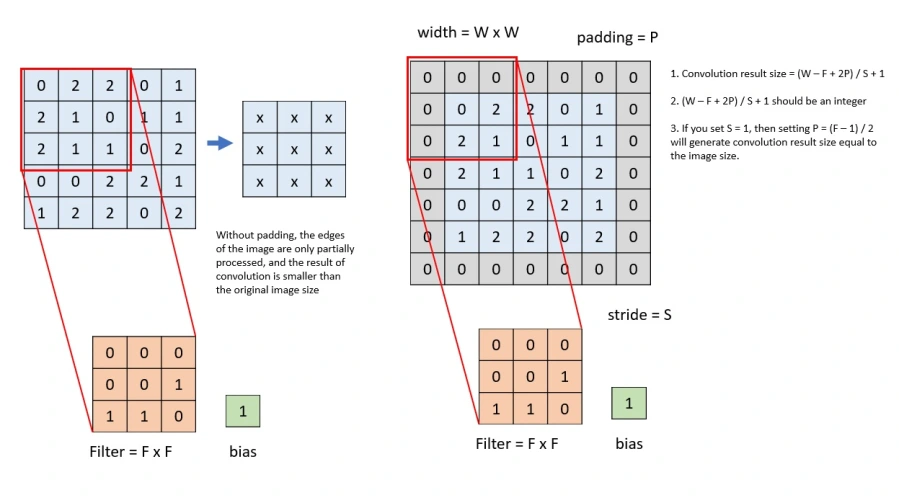
\includegraphics[width=0.95\textwidth,height=0.95\textheight,keepaspectratio]{images/convolutional-layer.png}
    \end{figure}

    \href{https://cs231n.github.io/convolutional-networks/}{Interactive demo: cs231n.github.io/convolutional-networks}
\end{frame}

\begin{frame}{Quick Exercise (5 mins)}
    \begin{block}{Let’s find out what this can give us:}
        \begin{itemize}
            \item Padding = 0
            \item Stride = 1
        \end{itemize}
    \end{block}
    \begin{figure}
    \centering
    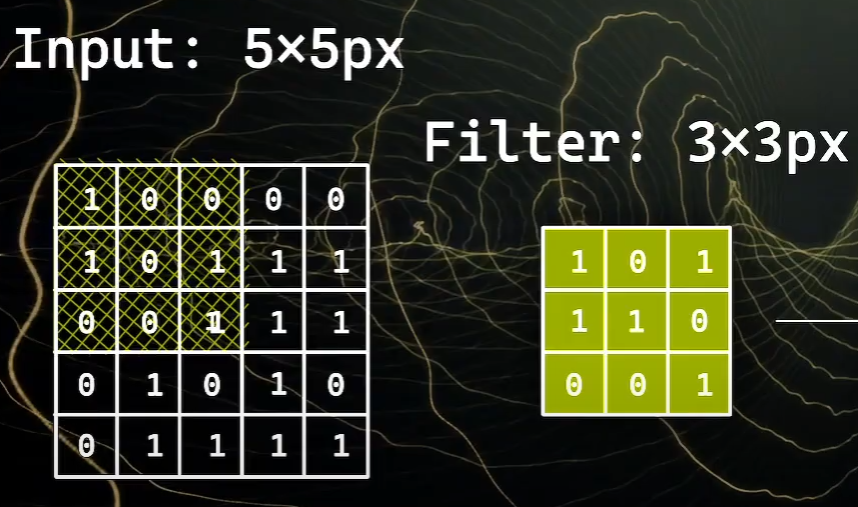
\includegraphics[width=0.7\textwidth,height=0.7\textheight,keepaspectratio]{images/cnn-exercise-1.png}
    \end{figure}

    Note: Once you traverse entire image/matrix it will give you a matrix calls Feature Map or Activation Map.
\end{frame}